\chapter{Statistical methods and optimisation techniques}\label{statistic_methods}

Gluck, Harris and Prado in the original BREACH paper investigated the attack on
stream ciphers such as RC4. They also suggested that block ciphers are vulnerable
without providing practical attack details. However, the use of RC4 is prohibited in
negotiation between servers and clients \cite{rc4_prohibit} due to several other major vulnerabili-
ties. 

Block alignment techniques have already been explored in the literature \cite{poodle} and 
Dimitris Karakostas also investigated statistical methods
to attack block ciphers in his thesis.
The section \ref{sec:blockalign} evolves the use of statistical
methods for block cipher attacks in a more structured way.

In the section \ref{sec:optimizations} we also propose various optimization techniques which
make the attack much more efficient.

\section{Block alignment}\label{sec:blockalign}

Block ciphers provide a greater challenge compared to stream ciphers, when it
comes to telling length apart, since stream ciphers provide better granularity. That
is because block ciphers round length to $\lambda$-bits, where $\lambda$ is the block size,
by adding padding.

In order to bypass this, we propose the introdution of artificial noise, 
which will force the creation of additional blocks, if necessary. 
Theoretically, it would be enough to issue $16\times$ more requests
to achieve block alignment. At this point, the correct candidate would result in one less
block, which in turn would provide a measurable length difference. 


\begin{figure}[H] \caption{Block Alginment} \centering
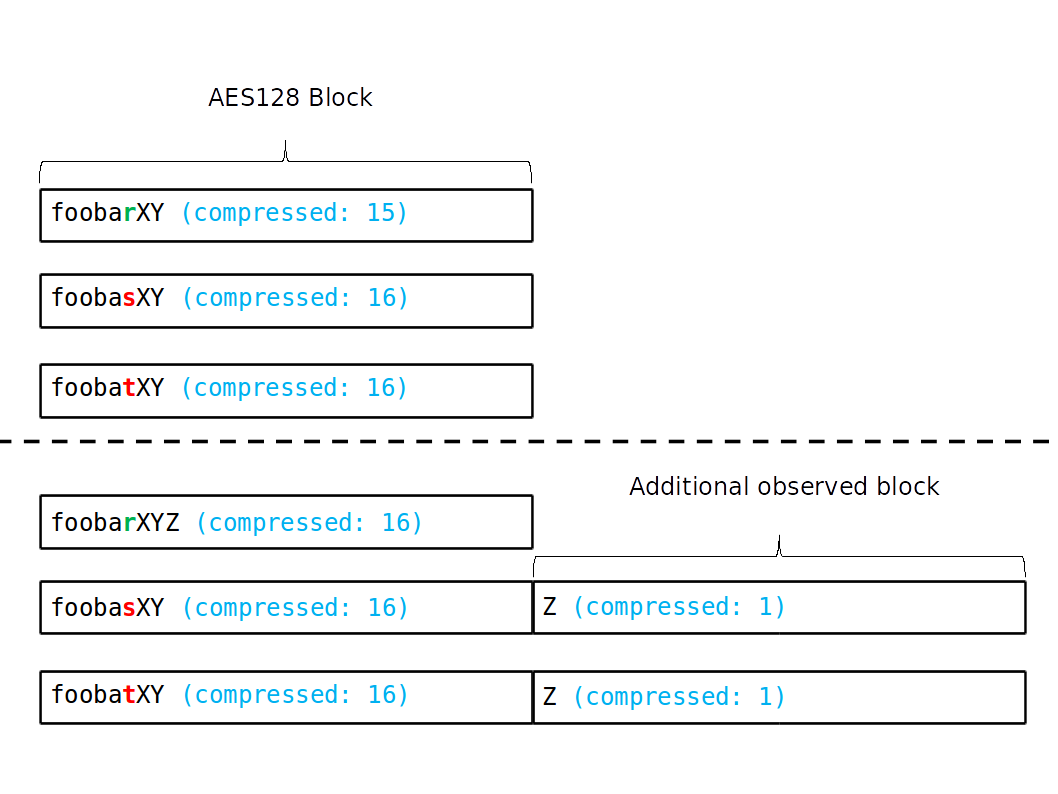
\includegraphics[width=0.7\textwidth]{diagrams/block_alignment.png}\end{figure}

This figure illusrates an example of how the artificial noise results in block alignment and 
how this contributes to distingush between lengths. The example assume a known secret
\textit{fooba} and a possible next byte drawn from the alphabet \textit{(r,s,t)}.
When the attack uses the padding \textit{XY}, the total lenght size 
of the three possible next bytes are the same. Although \textit{foobar} has 15 bits,
they are rounded up to 16 bits in respect of block alginment.
In case of padding \textit{XYZ}, the wrong candidates result in a one more block 
because they cross the block boundaries. Despite the actual difference of only 1 bit,
the use of block ciphers results in 16 bits length difference.


However, introduction of artificial noise is actually tricky. Firstly, noise should be carefully constructed
to avoid being compressed with itself. Secondly, each added symbol will alter the Huffman coding in a
different way, since the plaintext's symbol frequency distribution will be altered. It is advised to use symbols
which do not appear in the rest of the plaintext or they are rare. Even in this casee
 the Huffman tree will be expanded and, consequently, the length of the compressed text will increase,
 in a manner that cannot always be predicted.

\section{Optimizations}\label{sec:optimizations}


\subsection{Request soup}\label{subsec:soup}

A problem with encrypted responses is the fact that it is not possible to safely
determine which packet corresponds to which request, when requests are pipelined
by the browser. That way if the attacker was to issue
requests sequentially, they would have to ensure all response packets for each request
have arrived, before issuing the next one.

However, it is possible to avoid this delay, by making samplesets, each one containing multiple
requests for a specific symbol. For each sampleset, responses would then come pipelined and it
would not be possible to tell them apart. However, this does not indicate a problem since these requests
with the corresponding responses are not adaptive to each other and thus there is no
need to distinguish between then. The total length of the capture can still be
measured and divided by the known amount of requests that the sampleset
contains. This would be enough to calculate the desired mean length.
This statistical mean length converges to the sampleset distribution's mean length due to
the law of large numbers.

This method offers a speedup of up to $5\times$, considering a 200
ms delay and a 40 ms round trip time.



\subsection{Browser parallelization}

The optimization presented in section \ref{subsec:soup} would result in small benefit if no browser
parallelization was possible. Although the attacker would send multiple requests at the same time, the browser
would proceed them pipelined. 

Browsers allow in general up to 6 parallel HTTP requests, although this may differ depending
on the browser application and release. This allows issuing multiple parallel requests and
collecting samples at the same time, giving the attack a $6\times$ speedup.

Each parallel request cannot adapt based on previous results.
However, we need to collect multiple samples per candidate to perform
statistical analysis and extract the mean. These samples pertain to the same
candidate and can be collected non-adaptively.

\begin{figure}[H] \caption{Browser Parallelization} \centering
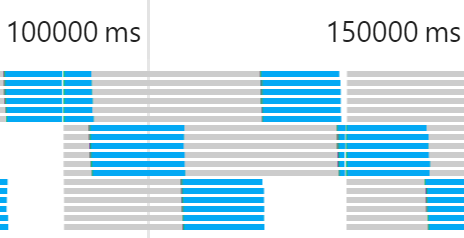
\includegraphics[width=0.7\textwidth]{diagrams/parallel.png}\end{figure}

